%% =====================================================================
%%  Case Study Report -- Cyber Security (Unit 4)
%%  AI-Powered Detection and Automated Response to Malicious PowerShell
%%  Attacks Using Machine Learning
%%
%%  Single-file Overleaf project (compile with pdfLaTeX). Before submitting,
%%  fill in the group number, names and roll numbers on the title page and
%%  save the PDF as G<group number>.pdf (for example, G10.pdf).
%% =====================================================================
\documentclass[12pt,a4paper]{article}

\usepackage[T1]{fontenc}
\usepackage[utf8]{inputenc}
\usepackage{lmodern}
\usepackage{mathptmx}                 % Times font
\usepackage[a4paper,margin=2.54cm]{geometry}
\usepackage{setspace}
\setstretch{1.3}
\usepackage{microtype}
\usepackage{amsmath}
\usepackage{array,booktabs,tabularx}
\usepackage{enumitem}
\setlist{itemsep=2pt,topsep=4pt}
\usepackage{cite}

\usepackage{xcolor}
\definecolor{navy}{HTML}{0D366B}
\definecolor{midblue}{HTML}{2A78D6}
\definecolor{paleblue}{HTML}{DCE7F5}

\usepackage{titlesec}
\titleformat{\section}{\normalfont\Large\bfseries\color{navy}}{\thesection}{0.7em}{}
\titleformat{\subsection}{\normalfont\large\bfseries\color{navy}}{\thesubsection}{0.7em}{}

\usepackage{caption}
\captionsetup{font=normalsize,labelfont={bf,color=navy},labelsep=colon}
\captionsetup[table]{position=top}

\usepackage{tikz}
\usetikzlibrary{positioning,arrows.meta}
\usepackage{pgfplots}
\pgfplotsset{compat=1.17}

\usepackage[hyphens]{url}
\usepackage[colorlinks=true,linkcolor=navy,citecolor=navy,urlcolor=navy]{hyperref}

\newcommand{\attck}{ATT\&CK}

\begin{document}

%% ---------------------------------------------------------------------
%%  Title page
%% ---------------------------------------------------------------------
\begin{titlepage}
  \centering
  \setstretch{1.15}
  {\large\textbf{CYBER SECURITY}\par}
  {Case Study Report (Unit 4)\par}
  \vspace{2.5cm}
  {\LARGE\bfseries\color{navy} AI-Powered Detection and Automated Response to Malicious PowerShell Attacks Using Machine Learning\par}
  \vspace{2cm}
  {\large\textbf{Group No.:} G\_\_\par}
  \vspace{0.6cm}
  \textbf{Topic Selected:} AI-Powered Detection and Automated Response to Malicious PowerShell Attacks Using Machine Learning\par
  \vspace{1.6cm}
  {\large\bfseries\color{navy} Group Members\par}
  \vspace{0.3cm}
  \begin{tabular}{c l l}
    \toprule
    \textbf{Sr. No.} & \textbf{Name of the Student} & \textbf{Roll No.}\\
    \midrule
    1 & [Student Name 1] & [Roll No.]\\
    2 & [Student Name 2] & [Roll No.]\\
    3 & [Student Name 3] & [Roll No.]\\
    4 & [Student Name 4] & [Roll No.]\\
    \bottomrule
  \end{tabular}\par
  \vfill
  Submitted to: [Name of the Faculty]\par
  [Department Name], [Name of the Institute]\par
  October 2026\par
\end{titlepage}

%% ---------------------------------------------------------------------
\section*{Abstract}
%% ---------------------------------------------------------------------
PowerShell is a scripting tool that comes with every Windows computer. Attackers often use it because it is trusted, powerful and can run code directly in memory without leaving files on disk. Traditional antivirus tools that look for fixed signatures find it hard to catch such scripts, because an attacker can easily change the text of a script while keeping its behaviour the same. This case study builds and tests a machine-learning system that reads a PowerShell script, decides whether it is malicious, and then takes an automatic response based on how risky the script is. We used the public MPSD dataset of malicious and benign PowerShell scripts. While preparing the data we found that more than half of the malicious files were exact copies, so duplicates were removed before training. We compared four machine-learning models and a simple ensemble. The ensemble achieved an F1-score of 0.972 and correctly detected 96.2\% of malicious scripts while wrongly flagging only 0.7\% of benign scripts. When tested on scripts it had never seen, the automatic response system contained 91.2\% of malicious scripts and wrongly blocked only 0.23\% of benign ones, taking about 91 milliseconds per script. The study shows that simple, explainable machine-learning models combined with a careful response policy can help organisations defend against PowerShell attacks.

\vspace{0.3cm}
\noindent\textbf{\color{navy}Keywords:} PowerShell, malware detection, machine learning, cyber attack, random forest, logistic regression, automated incident response, MITRE \attck{}.

\clearpage

%% ---------------------------------------------------------------------
\section{Introduction}
%% ---------------------------------------------------------------------

\subsection{Background}
PowerShell is a command-line shell and scripting language made by Microsoft. It is installed by default on Windows and is used by system administrators to automate everyday tasks such as managing users, installing software and changing settings. Because it is so powerful and is already trusted on the system, attackers also like to use it. With a single PowerShell command, an attacker can download harmful code from the internet and run it directly in memory, without saving any file on the disk. This type of attack is called a \emph{fileless} or \emph{living-off-the-land} attack, because the attacker uses tools that are already present on the computer~\cite{wueest2017}.

\subsection{Relevance of the Topic Today}
PowerShell attacks are a serious and current problem. Symantec reported that 95.4\% of the PowerShell scripts submitted to its analysis service were malicious~\cite{wueest2016}. MITRE \attck{}, a well-known knowledge base of attacker behaviour, lists PowerShell as technique T1059.001~\cite{mitre_t1059}, and the 2025 Threat Detection Report by Red Canary found that command and scripting interpreters were the most common attack technique for the sixth year in a row~\cite{redcanary2025}. Simply removing PowerShell is not possible, because organisations depend on it. In 2022, the NSA and CISA advised organisations to keep PowerShell but to log and monitor it carefully~\cite{nsa2022}.

Logging, however, only collects data; someone still has to decide whether each script is safe or harmful. Attackers make this harder by disguising their scripts with free tools such as Invoke-Obfuscation~\cite{bohannon2016}, and security teams already receive more alerts than they can check~\cite{hassan2019}. Machine learning can help by automatically scoring every script and allowing a fast and consistent response, which is in line with current incident-response guidance~\cite{nist2025}.

\subsection{Problem Statement}
Given the text of a PowerShell script captured on a Windows computer, the system should (1) decide whether the script is malicious, with very few false alarms, and (2) automatically take a suitable action, such as raising an alert or blocking the script, while leaving the most serious actions to a human analyst.

\subsection{Objectives}
\begin{enumerate}
  \item To prepare a clean and reliable dataset of malicious and benign PowerShell scripts.
  \item To extract useful features from the scripts and train machine-learning models to detect malicious ones.
  \item To compare the models and select the best one for detection.
  \item To design an automated response system that acts according to the risk level of each script.
  \item To test the complete system and discuss its strengths and limitations.
\end{enumerate}

%% ---------------------------------------------------------------------
\section{Literature Review}
%% ---------------------------------------------------------------------

\subsection{PowerShell Logging and Attack Knowledge}
Microsoft added security features to PowerShell that make detection possible. \emph{Script Block Logging} records the text of every script that runs as Windows Event ID 4104~\cite{ms_logging}, and the \emph{Antimalware Scan Interface} (AMSI) allows antivirus software to scan a script just before it runs~\cite{ms_amsi}. The MITRE \attck{} framework gives a common language to describe what an attacker is trying to do, such as downloading tools or stealing passwords~\cite{strom2018}. Security reports have described how attackers use PowerShell for downloading malware, moving across networks and staying hidden~\cite{wueest2016,wueest2017,redcanary2025}.

\subsection{Obfuscation and De-obfuscation}
Attackers often disguise (obfuscate) their scripts. Bohannon showed that a single command can be rewritten in many different forms~\cite{bohannon2016}, and Bohannon and Holmes later built Revoke-Obfuscation, which detects disguised scripts using statistical features~\cite{bohannon2017}. Several tools try to remove the disguise before analysis, including PowerDrive~\cite{ugarte2019}, the method of Li et al.~\cite{li2019} and its extension by Xiong et al.~\cite{xiong2022}, PowerDP~\cite{tsai2023} and PowerPeeler~\cite{li2024}. Recently, Patsakis et al.\ tested large language models (LLMs) and found that GPT-4 could recover hidden web addresses from real malicious scripts in about 70\% of cases~\cite{patsakis2024}.

\subsection{Machine Learning for PowerShell Detection}
Hendler et al.\ trained deep neural networks on more than 66,000 PowerShell commands and found that combining two different models gave the best results~\cite{hendler2018}. In later work they used AMSI data and reached a detection rate of nearly 90\% with less than 0.1\% false alarms~\cite{hendler2020}, and Microsoft described using such models in its Defender products~\cite{ms_blog2019}. Rusak et al.\ used the syntax tree of scripts~\cite{rusak2018}, Song et al.\ compared token-based and tree-based features and reported about 98\% detection~\cite{song2021}, and Mimura and Tajiri used word embeddings~\cite{mimura2021}. Fang et al.\ combined several types of features with a random forest, reported 98.93\% accuracy and released the MPSD dataset used in this study~\cite{fang2021}. Saxe and Berlin showed that character-level models work well for short security texts such as web addresses~\cite{saxe2017}. General reviews of machine learning for malware are given by Ucci et al.~\cite{ucci2019} and Gibert et al.~\cite{gibert2020}. The newest work uses LLMs to both detect and explain malicious PowerShell~\cite{wang2026}.

\subsection{Evaluation Problems and Automated Response}
Researchers have warned that machine-learning results in security can look better than they really are. Sommer and Paxson explained why intrusion detection is harder than normal classification tasks~\cite{sommer2010}. Arp et al.\ listed common mistakes, such as letting very similar samples appear in both training and test data~\cite{arp2022}, and Pendlebury et al.\ showed that careless data splitting can make malware detectors look much more accurate than they are~\cite{pendlebury2019}. On the response side, security orchestration and automation (SOAR) tools connect detection to automatic actions~\cite{islam2019}, and provenance-based methods help analysts deal with large numbers of alerts~\cite{hassan2019,hassan2020}.

\subsection{Summary and Research Gap}
Table~\ref{tab:lit} summarises some important studies. Most previous work focuses only on detection and reports very high accuracy, but few studies check their datasets for duplicate samples, and very few connect the detection result to an automatic response. This case study addresses both points.

\begin{table}[htbp]
\centering
\caption{Summary of related work}\label{tab:lit}
\begin{tabularx}{\textwidth}{>{\raggedright\arraybackslash}p{3.3cm} >{\raggedright\arraybackslash}X >{\raggedright\arraybackslash}p{4.3cm}}
\toprule
\textbf{Study} & \textbf{Method} & \textbf{Result}\\
\midrule
Hendler et al.~\cite{hendler2018} & Deep neural networks on PowerShell commands & High detection, very few false alarms\\
Hendler et al.~\cite{hendler2020} & AMSI data with pre-trained embeddings & About 90\% detection\\
Bohannon \& Holmes~\cite{bohannon2017} & Statistical features to detect obfuscation & Robust obfuscation detection\\
Song et al.~\cite{song2021} & Token and syntax-tree features & About 98\% detection\\
Fang et al.~\cite{fang2021} & Hybrid features with random forest & 98.93\% accuracy\\
Wang et al.~\cite{wang2026} & Large language models & Detection with explanations\\
\bottomrule
\end{tabularx}
\end{table}

%% ---------------------------------------------------------------------
\section{Methodology}
%% ---------------------------------------------------------------------

\subsection{Overview}
The proposed system works in six steps, shown in Figure~\ref{fig:flow}. First, the text of each PowerShell script is collected from Windows logs. The data is then cleaned, useful features are extracted, and a machine-learning model gives each script a risk score between 0 and 1. Finally, a response policy uses the score to choose an action, and every decision is recorded.

\begin{figure}[htbp]
\centering
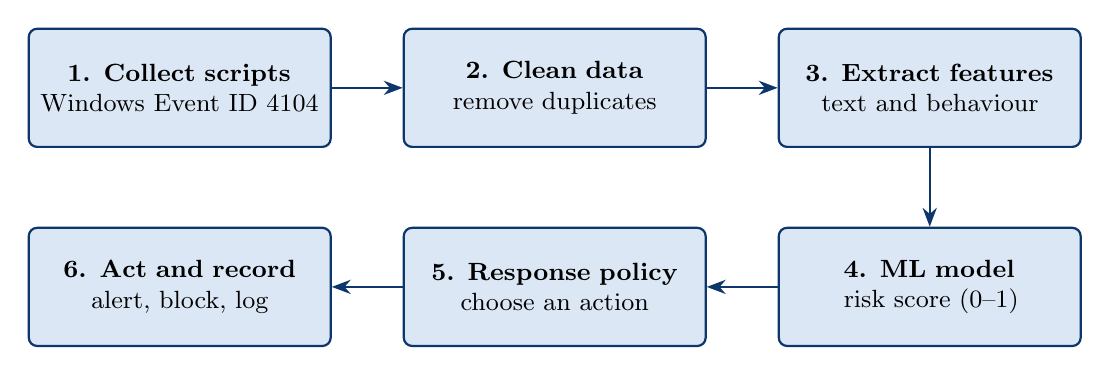
\begin{tikzpicture}[font=\small,
  box/.style={draw=navy, thick, rounded corners=3pt, fill=paleblue, align=center, text width=3.6cm, minimum height=1.5cm},
  arr/.style={-{Stealth[length=2.4mm]}, thick, navy}]
  \node[box] (a) {\textbf{1. Collect scripts}\\ Windows Event ID 4104};
  \node[box, right=0.9cm of a] (b) {\textbf{2. Clean data}\\ remove duplicates};
  \node[box, right=0.9cm of b] (c) {\textbf{3. Extract features}\\ text and behaviour};
  \node[box, below=1.0cm of c] (d) {\textbf{4. ML model}\\ risk score (0--1)};
  \node[box, left=0.9cm of d] (e) {\textbf{5. Response policy}\\ choose an action};
  \node[box, left=0.9cm of e] (f) {\textbf{6. Act and record}\\ alert, block, log};
  \draw[arr] (a) -- (b); \draw[arr] (b) -- (c); \draw[arr] (c) -- (d);
  \draw[arr] (d) -- (e); \draw[arr] (e) -- (f);
\end{tikzpicture}
\caption{Workflow of the proposed system}\label{fig:flow}
\end{figure}

\subsection{Dataset}
We used the public MPSD dataset released by Fang et al.~\cite{fang2021}. It contains 4,202 malicious scripts, 4,316 benign scripts and 4,202 ``mixed'' scripts in which malicious code is hidden inside a normal script. The malicious scripts include downloaders, shellcode loaders, reverse shells and password-stealing tools. The benign scripts are normal administration scripts collected from public sources. All malicious scripts were treated only as text and were never run.

\subsection{Data Cleaning}
Before training, the data was checked for problems, as recommended by Arp et al.~\cite{arp2022}:
\begin{itemize}
  \item \textbf{Duplicates:} only 1,875 of the 4,202 malicious files were unique, which means 55.2\% were exact copies. Duplicates were removed so that every script is counted only once.
  \item \textbf{Wrong labels:} 12 files appeared in both the malicious and benign folders. As their true label is unknown, they were removed.
  \item \textbf{Hidden shortcut:} a special byte-order mark appeared at the start of about 35\% of benign files but never in malicious files. A model could learn this meaningless pattern, so it was removed from all files.
  \item \textbf{Near-copies:} many malicious scripts differ only in variable names or numbers. Such near-copies were grouped into ``families'' (816 families for 1,875 malicious scripts), so that a family is never split between training and testing.
\end{itemize}
After cleaning, 1,875 malicious and 4,302 benign scripts remained.

\subsection{Feature Extraction}
Each script is first converted to lower case and the backtick character (\verb|`|) is removed, because PowerShell ignores both and attackers use them to disguise commands. Two kinds of features are then extracted:
\begin{enumerate}
  \item \textbf{Text features (TF-IDF):} the script is split into short sequences of 3 to 5 characters, and each sequence is given a weight using TF-IDF~\cite{salton1988}. A sequence gets a high weight if it appears often in a script but rarely in other scripts:
  \begin{equation}
    \text{TF-IDF}(t,d) = \text{tf}(t,d) \times \log\frac{N}{\text{df}(t)},
  \end{equation}
  where $\text{tf}(t,d)$ is how often sequence $t$ appears in script $d$, $N$ is the number of scripts and $\text{df}(t)$ is the number of scripts that contain $t$.
  \item \textbf{Behaviour and statistical features (33 features):} simple measurements such as script length, number of lines, randomness of characters (entropy), and counts of suspicious keywords. The keywords are grouped by attacker behaviour and linked to MITRE \attck{}, for example \texttt{DownloadString} (downloading tools, T1105), \texttt{Invoke-Expression} (running code, T1059.001) and \texttt{VirtualAlloc} (code injection, T1055).
\end{enumerate}

\subsection{Machine-Learning Models}
Four models and one ensemble were trained using the scikit-learn library~\cite{pedregosa2011}:
\begin{itemize}
  \item \textbf{Logistic Regression (LR) on text features:} a simple and fast linear model that works well with large numbers of text features.
  \item \textbf{Logistic Regression on behaviour features:} a simple baseline.
  \item \textbf{Random Forest (RF) on behaviour features:} a group of 300 decision trees that vote together~\cite{breiman2001}; it can learn complex patterns and is robust.
  \item \textbf{Gradient Boosting (HGB) on behaviour features:} a strong tree-based model similar to LightGBM~\cite{ke2017}.
  \item \textbf{Ensemble:} the average of the LR (text) and RF (behaviour) scores. The two models look at different evidence, so combining them makes the result more stable.
\end{itemize}
Deep learning was not used because the dataset is small (about 6,000 scripts) and simpler models are faster and easier to explain.

\subsection{Evaluation}
The models were tested using five-fold cross-validation~\cite{kohavi1995}: the data is split into five parts, and each part is used once for testing while the other four are used for training. Families of near-copies were always kept in the same part, so a model is never tested on a script it has almost seen before. The following measures were used, where TP, FP, TN and FN are true positives, false positives, true negatives and false negatives:
\begin{equation}
  \text{Precision} = \frac{TP}{TP+FP},\qquad \text{Recall} = \frac{TP}{TP+FN},\qquad F_1 = \frac{2 \times \text{Precision} \times \text{Recall}}{\text{Precision} + \text{Recall}}.
\end{equation}
Accuracy and the area under the ROC curve (AUC) were also reported.

\subsection{Automated Response}
The risk score from the model is used to choose one of four actions, as shown in Table~\ref{tab:tiers}. Less harmful actions are taken automatically, while the most serious action, disconnecting a computer from the network, needs approval from a human analyst. Every decision is saved in a log file, and suspicious web addresses are written in a safe form (for example, \texttt{hxxp} instead of \texttt{http}).

\begin{table}[htbp]
\centering
\caption{Response levels used by the system}\label{tab:tiers}
\begin{tabularx}{\textwidth}{>{\raggedright\arraybackslash}p{2.2cm} >{\raggedright\arraybackslash}p{3.6cm} >{\raggedright\arraybackslash}X}
\toprule
\textbf{Level} & \textbf{Risk score} & \textbf{Action}\\
\midrule
Allow & below 0.30 & Record the result only\\
Alert & 0.30 to 0.70 & Send an alert to the security team with details\\
Contain & 0.70 or above & Stop the script, quarantine the file and block its web addresses\\
Isolate & 0.95 or above, with dangerous behaviour & Disconnect the computer from the network after analyst approval\\
\bottomrule
\end{tabularx}
\end{table}

%% ---------------------------------------------------------------------
\section{Implementation Details}
%% ---------------------------------------------------------------------
The system was written in Python. Table~\ref{tab:tools} lists the main tools.

\begin{table}[htbp]
\centering
\caption{Tools and environment}\label{tab:tools}
\begin{tabular}{ll}
\toprule
\textbf{Item} & \textbf{Details}\\
\midrule
Programming language & Python 3.13\\
Machine-learning library & scikit-learn 1.9\\
Data handling & pandas, NumPy\\
Graphs & Matplotlib\\
Hardware & 4-core CPU, 15 GB RAM (no GPU)\\
Dataset & MPSD (public, GitHub)~\cite{fang2021}\\
\bottomrule
\end{tabular}
\end{table}

The code is divided into four main parts:
\begin{enumerate}
  \item \textbf{Data module:} reads the scripts, removes duplicates and wrong labels, and groups near-copies into families.
  \item \textbf{Feature module:} cleans the text and calculates the text and behaviour features.
  \item \textbf{Model module:} trains and tests the models and the ensemble.
  \item \textbf{Response module:} reads Windows Event ID 4104 records, gets a risk score from the model, chooses the response level, adds the matching \attck{} technique and writes the decision to a log. For safety, it runs in a test (dry-run) mode where actions are recorded but not actually carried out.
\end{enumerate}
In a real organisation, Script Block Logging would be switched on through Group Policy~\cite{ms_logging}, the logs would be sent to a central server for scoring, and the response module would be connected to the company's security tools. Seven unit tests were written to check the main functions, and all of them pass.

%% ---------------------------------------------------------------------
\section{Results and Discussion}
%% ---------------------------------------------------------------------

\subsection{Model Performance}
Table~\ref{tab:results} shows the results of all models, and Figure~\ref{fig:f1} compares their F1-scores. All models performed well, which shows that malicious and benign PowerShell scripts are clearly different. The text-based LR model had the highest F1-score (0.974), and the ensemble was almost the same (0.972) but produced the fewest false alarms among the high-scoring models (30 compared with 37). Since false alarms can stop legitimate work, the ensemble was chosen for the response system. The behaviour-only LR model was the weakest, which shows that tree-based models capture patterns that a simple linear model misses.

\begin{table}[htbp]
\centering
\caption{Performance of the models (five-fold cross-validation)}\label{tab:results}
\begin{tabular}{lccccc}
\toprule
\textbf{Model} & \textbf{Accuracy} & \textbf{Precision} & \textbf{Recall} & \textbf{F1} & \textbf{AUC}\\
\midrule
LR (behaviour)        & 0.974 & 0.953 & 0.960 & 0.957 & 0.988\\
RF (behaviour)        & 0.980 & 0.982 & 0.952 & 0.967 & 0.995\\
HGB (behaviour)       & 0.979 & 0.984 & 0.948 & 0.966 & 0.996\\
LR (text, TF-IDF)     & 0.985 & 0.980 & 0.969 & 0.974 & 0.999\\
Ensemble (LR + RF)    & 0.984 & 0.984 & 0.962 & 0.972 & 0.998\\
\bottomrule
\end{tabular}
\end{table}

\begin{figure}[htbp]
\centering
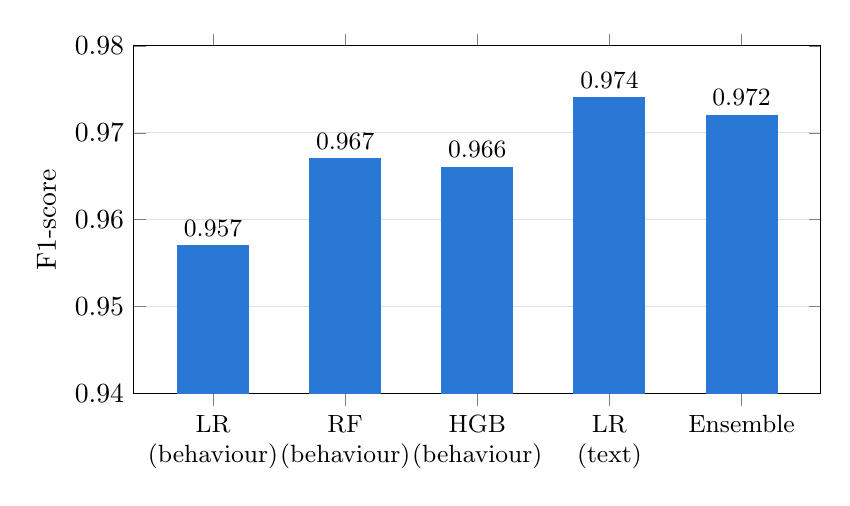
\begin{tikzpicture}
\begin{axis}[ybar, width=0.85\textwidth, height=6cm, bar width=0.9cm, ymin=0.94, ymax=0.98,
  symbolic x coords={LR (behaviour),RF (behaviour),HGB (behaviour),LR (text),Ensemble},
  xtick=data, xticklabels={{LR\\(behaviour)},{RF\\(behaviour)},{HGB\\(behaviour)},{LR\\(text)},{Ensemble}}, x tick label style={font=\small, align=center},
  ylabel={F1-score}, nodes near coords, every node near coord/.append style={font=\small, /pgf/number format/fixed, /pgf/number format/precision=3},
  yticklabel style={/pgf/number format/fixed, /pgf/number format/precision=2},
  ymajorgrids, grid style={black!12}, enlarge x limits=0.15]
\addplot[fill=midblue, draw=midblue] coordinates {(LR (behaviour),0.957) (RF (behaviour),0.967) (HGB (behaviour),0.966) (LR (text),0.974) (Ensemble,0.972)};
\end{axis}
\end{tikzpicture}
\caption{F1-score of each model}\label{fig:f1}
\end{figure}

Figure~\ref{fig:cm} shows the confusion matrix of the ensemble. Out of 4,302 benign scripts, 4,272 (99.3\%) were correctly classified, and out of 1,875 malicious scripts, 1,803 (96.2\%) were correctly detected.

\begin{figure}[htbp]
\centering
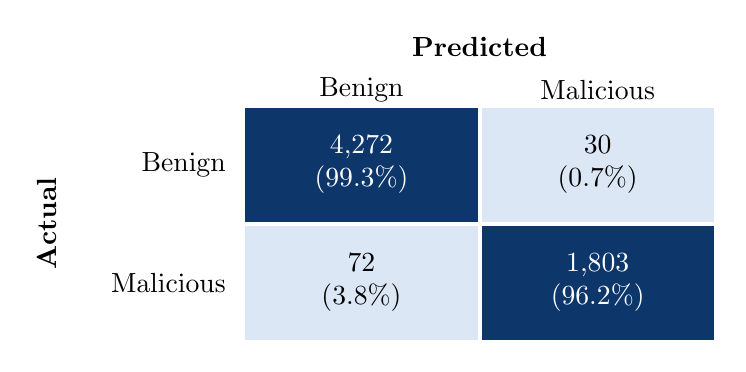
\begin{tikzpicture}[cell/.style={minimum width=3.0cm, minimum height=1.5cm, draw=white, line width=1.5pt, align=center}]
  \node[cell, fill=navy, text=white] at (0,0) {4,272\\(99.3\%)};
  \node[cell, fill=paleblue] at (3.0,0) {30\\(0.7\%)};
  \node[cell, fill=paleblue] at (0,-1.5) {72\\(3.8\%)};
  \node[cell, fill=navy, text=white] at (3.0,-1.5) {1,803\\(96.2\%)};
  \node[anchor=east] at (-1.6,0) {Benign};
  \node[anchor=east] at (-1.6,-1.5) {Malicious};
  \node at (0,0.95) {Benign};
  \node at (3.0,0.95) {Malicious};
  \node[font=\bfseries] at (1.5,1.5) {Predicted};
  \node[font=\bfseries, rotate=90] at (-4.0,-0.75) {Actual};
\end{tikzpicture}
\caption{Confusion matrix of the ensemble model}\label{fig:cm}
\end{figure}

\subsection{Effect of Removing Duplicates}
To see why data cleaning matters, the ensemble was also tested on the original data with duplicates and a simple random split. In that case its F1-score rose to 0.988 and the share of missed malicious scripts fell from 3.8\% to 1.7\%. This higher result is misleading, because the model was partly being tested on copies of scripts it had already seen. In other words, without cleaning, the number of attacks missed in real use would be underestimated by more than half. This agrees with the warnings of Arp et al.~\cite{arp2022} and Pendlebury et al.~\cite{pendlebury2019}.

\subsection{Malicious Code Hidden Inside Normal Scripts}
The models were also tested on the ``mixed'' scripts, where malicious code is hidden inside a long normal script. This was the main weakness found: the ensemble detected only 46.7\% of these scripts, because the large amount of normal code hides the small malicious part. When examples of mixed scripts were added to the training data, detection rose to 96.4\%, while false alarms on normal scripts increased only slightly (from 0.70\% to 1.05\%). Training with such examples is therefore recommended.

\subsection{Automated Response Results}
To test the full system, the ensemble was trained on four parts of the data, and the fifth part (1,233 scripts it had never seen) was sent through the response system as Windows log events. Table~\ref{tab:response} shows the outcome. Most malicious scripts were stopped automatically, very few benign scripts were blocked, and a typical script was processed in about 91 milliseconds. The most common attacker behaviours found were running code with PowerShell (T1059.001), loading code into memory (T1620), code injection (T1055) and downloading tools (T1105).

\begin{table}[htbp]
\centering
\caption{Results of the automated response test}\label{tab:response}
\begin{tabular}{lr}
\toprule
\textbf{Measure} & \textbf{Result}\\
\midrule
Scripts tested (malicious / benign) & 373 / 860\\
Malicious scripts stopped automatically & 91.2\%\\
Malicious scripts at least alerted & 97.1\%\\
Benign scripts wrongly blocked & 0.23\% (2 scripts)\\
Benign scripts sent as alerts & 0.81\%\\
Average time per script (median) & 90.7 ms\\
\bottomrule
\end{tabular}
\end{table}

\subsection{Limitations}
The study has some limitations. Only one public dataset was used, so results should be checked again on real company data. The system looks only at the script text and not at other information such as which program started the script. Most mistakes were made on scripts that can be used for both good and bad purposes, such as system tools that also use low-level Windows functions. Finally, the response actions were tested in a safe simulation, not on a real network.

%% ---------------------------------------------------------------------
\section{Conclusion}
%% ---------------------------------------------------------------------
This case study showed that machine learning can detect malicious PowerShell scripts accurately and support a fast automatic response. After removing duplicates and wrong labels from the MPSD dataset, an ensemble of a text-based logistic regression model and a behaviour-based random forest reached an F1-score of 0.972, detecting 96.2\% of malicious scripts with only 0.7\% false alarms. The automated response system stopped 91.2\% of malicious scripts in a test on unseen data, wrongly blocked only 0.23\% of benign scripts, and needed about 91 milliseconds per script. Two lessons stand out: datasets must be checked for duplicates, otherwise results look better than they are, and malicious code hidden inside normal scripts needs special training data. In future, the system can be improved by testing it on real company logs, scanning scripts before they run using AMSI, adding information about running processes, and using large language models to explain alerts to analysts~\cite{wang2026}. Overall, simple and explainable models together with a careful, human-supervised response policy offer a practical defence against PowerShell attacks, in line with expert guidance to keep PowerShell but monitor it closely~\cite{nsa2022}.

%% ---------------------------------------------------------------------
%%  References
%% ---------------------------------------------------------------------
\setstretch{1.05}
\begin{thebibliography}{99}

\bibitem{wueest2017} C.~Wueest and H.~Anand, ``Living off the land and fileless attack techniques,'' Symantec Internet Security Threat Report (ISTR) Special Report, Symantec Corp., Jul. 2017.

\bibitem{wueest2016} C.~Wueest, ``The increased use of PowerShell in attacks,'' Symantec Security Response White Paper, Symantec Corp., Oct. 2016.

\bibitem{mitre_t1059} The MITRE Corporation, ``Command and Scripting Interpreter: PowerShell (T1059.001),'' \emph{MITRE ATT\&CK}. [Online]. Available: \url{https://attack.mitre.org/techniques/T1059/001/}

\bibitem{redcanary2025} Red Canary, ``2025 Threat Detection Report,'' Red Canary Inc., Denver, CO, USA, 2025. [Online]. Available: \url{https://redcanary.com/threat-detection-report/}

\bibitem{nsa2022} National Security Agency, Cybersecurity and Infrastructure Security Agency, New Zealand National Cyber Security Centre and UK National Cyber Security Centre, ``Keeping PowerShell: Security measures to use and embrace,'' Joint Cybersecurity Information Sheet, Jun. 2022.

\bibitem{bohannon2016} D.~Bohannon, ``Invoke-Obfuscation: PowerShell command and script obfuscator,'' presented at DerbyCon 6.0, Louisville, KY, USA, 2016. [Online]. Available: \url{https://github.com/danielbohannon/Invoke-Obfuscation}

\bibitem{hassan2019} W.~U. Hassan, S.~Guo, D.~Li, Z.~Chen, K.~Jee, Z.~Li and A.~Bates, ``NoDoze: Combatting threat alert fatigue with automated provenance triage,'' in \emph{Proc. Network and Distributed System Security Symp. (NDSS)}, San Diego, CA, USA, 2019.

\bibitem{nist2025} A.~Nelson, S.~Rekhi, M.~Souppaya and K.~Scarfone, ``Incident response recommendations and considerations for cybersecurity risk management: A CSF 2.0 community profile,'' NIST Special Publication 800-61 Rev.~3, National Institute of Standards and Technology, Gaithersburg, MD, USA, Apr. 2025.

\bibitem{ms_logging} Microsoft, ``about\_Logging\_Windows,'' PowerShell Documentation, Microsoft Learn. [Online]. Available: \url{https://learn.microsoft.com/en-us/powershell/module/microsoft.powershell.core/about/about_logging_windows}

\bibitem{ms_amsi} Microsoft, ``Antimalware Scan Interface (AMSI),'' Win32 Apps Documentation, Microsoft Learn. [Online]. Available: \url{https://learn.microsoft.com/en-us/windows/win32/amsi/antimalware-scan-interface-portal}

\bibitem{strom2018} B.~E. Strom, A.~Applebaum, D.~P. Miller, K.~C. Nickels, A.~G. Pennington and C.~B. Thomas, ``MITRE ATT\&CK: Design and philosophy,'' The MITRE Corporation, McLean, VA, USA, Tech. Rep. MTR180360, 2018.

\bibitem{bohannon2017} D.~Bohannon and L.~Holmes, ``Revoke-Obfuscation: PowerShell obfuscation detection using science,'' White Paper, Black Hat USA, Las Vegas, NV, USA, Jul. 2017.

\bibitem{ugarte2019} D.~Ugarte, D.~Maiorca, F.~Cara and G.~Giacinto, ``PowerDrive: Accurate de-obfuscation and analysis of PowerShell malware,'' in \emph{Detection of Intrusions and Malware, and Vulnerability Assessment (DIMVA 2019)}, Lecture Notes in Computer Science, vol.~11543. Cham, Switzerland: Springer, 2019, pp.~240--259.

\bibitem{li2019} Z.~Li, Q.~A. Chen, C.~Xiong, Y.~Chen, T.~Zhu and H.~Yang, ``Effective and light-weight deobfuscation and semantic-aware attack detection for PowerShell scripts,'' in \emph{Proc. ACM SIGSAC Conf. Computer and Communications Security (CCS)}, London, UK, 2019, pp.~1831--1847.

\bibitem{xiong2022} C.~Xiong, Z.~Li, Y.~Chen, T.~Zhu, J.~Wang, H.~Yang and W.~Ruan, ``Generic, efficient, and effective deobfuscation and semantic-aware attack detection for PowerShell scripts,'' \emph{Frontiers of Information Technology \& Electronic Engineering}, vol.~23, no.~3, pp.~361--381, 2022.

\bibitem{tsai2023} M.-H. Tsai, C.-C. Lin, Z.-G. He, W.-C. Yang and C.-L. Lei, ``PowerDP: De-obfuscating and profiling malicious PowerShell commands with multi-label classifiers,'' \emph{IEEE Access}, vol.~11, 2023.

\bibitem{li2024} R.~Li, C.~Zhang, H.~Chai, L.~Ying, H.~Duan and J.~Tao, ``PowerPeeler: A precise and general dynamic deobfuscation method for PowerShell scripts,'' in \emph{Proc. ACM SIGSAC Conf. Computer and Communications Security (CCS '24)}, Salt Lake City, UT, USA, 2024.

\bibitem{patsakis2024} C.~Patsakis, F.~Casino and N.~Lykousas, ``Assessing LLMs in malicious code deobfuscation of real-world malware campaigns,'' \emph{Expert Systems with Applications}, vol.~256, Art. no.~124912, 2024.

\bibitem{hendler2018} D.~Hendler, S.~Kels and A.~Rubin, ``Detecting malicious PowerShell commands using deep neural networks,'' in \emph{Proc. ACM Asia Conf. Computer and Communications Security (ASIACCS)}, Incheon, Republic of Korea, 2018, pp.~187--197.

\bibitem{hendler2020} D.~Hendler, S.~Kels and A.~Rubin, ``AMSI-based detection of malicious PowerShell code using contextual embeddings,'' in \emph{Proc. 15th ACM Asia Conf. Computer and Communications Security (ASIA CCS '20)}, Taipei, Taiwan, 2020, pp.~679--693.

\bibitem{ms_blog2019} Microsoft Defender Research Team, ``Deep learning rises: New methods for detecting malicious PowerShell,'' Microsoft Security Blog, Sep. 3, 2019. [Online]. Available: \url{https://www.microsoft.com/en-us/security/blog/2019/09/03/deep-learning-rises-new-methods-for-detecting-malicious-powershell/}

\bibitem{rusak2018} G.~Rusak, A.~Al-Dujaili and U.-M. O'Reilly, ``AST-based deep learning for detecting malicious PowerShell,'' in \emph{Proc. ACM SIGSAC Conf. Computer and Communications Security (CCS)}, Toronto, ON, Canada, 2018, pp.~2276--2278.

\bibitem{song2021} J.~Song, J.~Kim, S.~Choi, J.~Kim and I.~Kim, ``Evaluations of AI-based malicious PowerShell detection with feature optimizations,'' \emph{ETRI Journal}, vol.~43, no.~3, pp.~549--560, 2021.

\bibitem{mimura2021} M.~Mimura and Y.~Tajiri, ``Static detection of malicious PowerShell based on word embeddings,'' \emph{Internet of Things}, vol.~15, Art. no.~100404, 2021.

\bibitem{fang2021} Y.~Fang, X.~Zhou and C.~Huang, ``Effective method for detecting malicious PowerShell scripts based on hybrid features,'' \emph{Neurocomputing}, vol.~448, pp.~30--39, 2021.

\bibitem{saxe2017} J.~Saxe and K.~Berlin, ``eXpose: A character-level convolutional neural network with embeddings for detecting malicious URLs, file paths and registry keys,'' arXiv preprint arXiv:1702.08568, 2017.

\bibitem{ucci2019} D.~Ucci, L.~Aniello and R.~Baldoni, ``Survey of machine learning techniques for malware analysis,'' \emph{Computers \& Security}, vol.~81, pp.~123--147, 2019.

\bibitem{gibert2020} D.~Gibert, C.~Mateu and J.~Planes, ``The rise of machine learning for detection and classification of malware: Research developments, trends and challenges,'' \emph{Journal of Network and Computer Applications}, vol.~153, Art. no.~102526, 2020.

\bibitem{wang2026} M.~Wang, E.~Topolovec, B.~Arana, N.~V.~P.~S.~G.~C.~Kuladeep, Z.~Xi, G.~Yan, X.~Shu, S.~D.~Stoller and P.~Yang, ``Detection and explanation of PowerShell malware with large language models,'' Manuscript, Binghamton University, IBM T.~J. Watson Research Center and Stony Brook University, 2026.

\bibitem{sommer2010} R.~Sommer and V.~Paxson, ``Outside the closed world: On using machine learning for network intrusion detection,'' in \emph{Proc. IEEE Symp. Security and Privacy}, Oakland, CA, USA, 2010, pp.~305--316.

\bibitem{arp2022} D.~Arp, E.~Quiring, F.~Pendlebury, A.~Warnecke, F.~Pierazzi, C.~Wressnegger, L.~Cavallaro and K.~Rieck, ``Dos and don'ts of machine learning in computer security,'' in \emph{Proc. 31st USENIX Security Symp.}, Boston, MA, USA, 2022, pp.~3971--3988.

\bibitem{pendlebury2019} F.~Pendlebury, F.~Pierazzi, R.~Jordaney, J.~Kinder and L.~Cavallaro, ``TESSERACT: Eliminating experimental bias in malware classification across space and time,'' in \emph{Proc. 28th USENIX Security Symp.}, Santa Clara, CA, USA, 2019, pp.~729--746.

\bibitem{islam2019} C.~Islam, M.~A. Babar and S.~Nepal, ``A multi-vocal review of security orchestration,'' \emph{ACM Computing Surveys}, vol.~52, no.~2, Art. no.~37, 2019.

\bibitem{hassan2020} W.~U. Hassan, A.~Bates and D.~Marino, ``Tactical provenance analysis for endpoint detection and response systems,'' in \emph{Proc. IEEE Symp. Security and Privacy (S\&P)}, San Francisco, CA, USA, 2020, pp.~1172--1189.

\bibitem{salton1988} G.~Salton and C.~Buckley, ``Term-weighting approaches in automatic text retrieval,'' \emph{Information Processing \& Management}, vol.~24, no.~5, pp.~513--523, 1988.

\bibitem{pedregosa2011} F.~Pedregosa \emph{et al.}, ``Scikit-learn: Machine learning in Python,'' \emph{Journal of Machine Learning Research}, vol.~12, pp.~2825--2830, 2011.

\bibitem{breiman2001} L.~Breiman, ``Random forests,'' \emph{Machine Learning}, vol.~45, no.~1, pp.~5--32, 2001.

\bibitem{ke2017} G.~Ke, Q.~Meng, T.~Finley, T.~Wang, W.~Chen, W.~Ma, Q.~Ye and T.-Y. Liu, ``LightGBM: A highly efficient gradient boosting decision tree,'' in \emph{Advances in Neural Information Processing Systems 30 (NeurIPS)}, 2017, pp.~3146--3154.

\bibitem{kohavi1995} R.~Kohavi, ``A study of cross-validation and bootstrap for accuracy estimation and model selection,'' in \emph{Proc. 14th Int. Joint Conf. Artificial Intelligence (IJCAI)}, Montreal, QC, Canada, 1995, pp.~1137--1143.

\end{thebibliography}

\end{document}
